\subsection{Descrição do bloco de controle}

O bloco de controle é composto por 12 estados chamados de \verb|initial|,
\verb|load_memory|, \verb|iterate_lm|, \verb|acc_reset|,
\verb|arith|, \verb|iterate_arith|, \verb|acc_load|, \verb|sqrt|,
\verb|iterate_sqrt|, \verb|result_load|, \verb|iterate| e 
\verb|final|.

\begin{figure}[!hb]
\centering
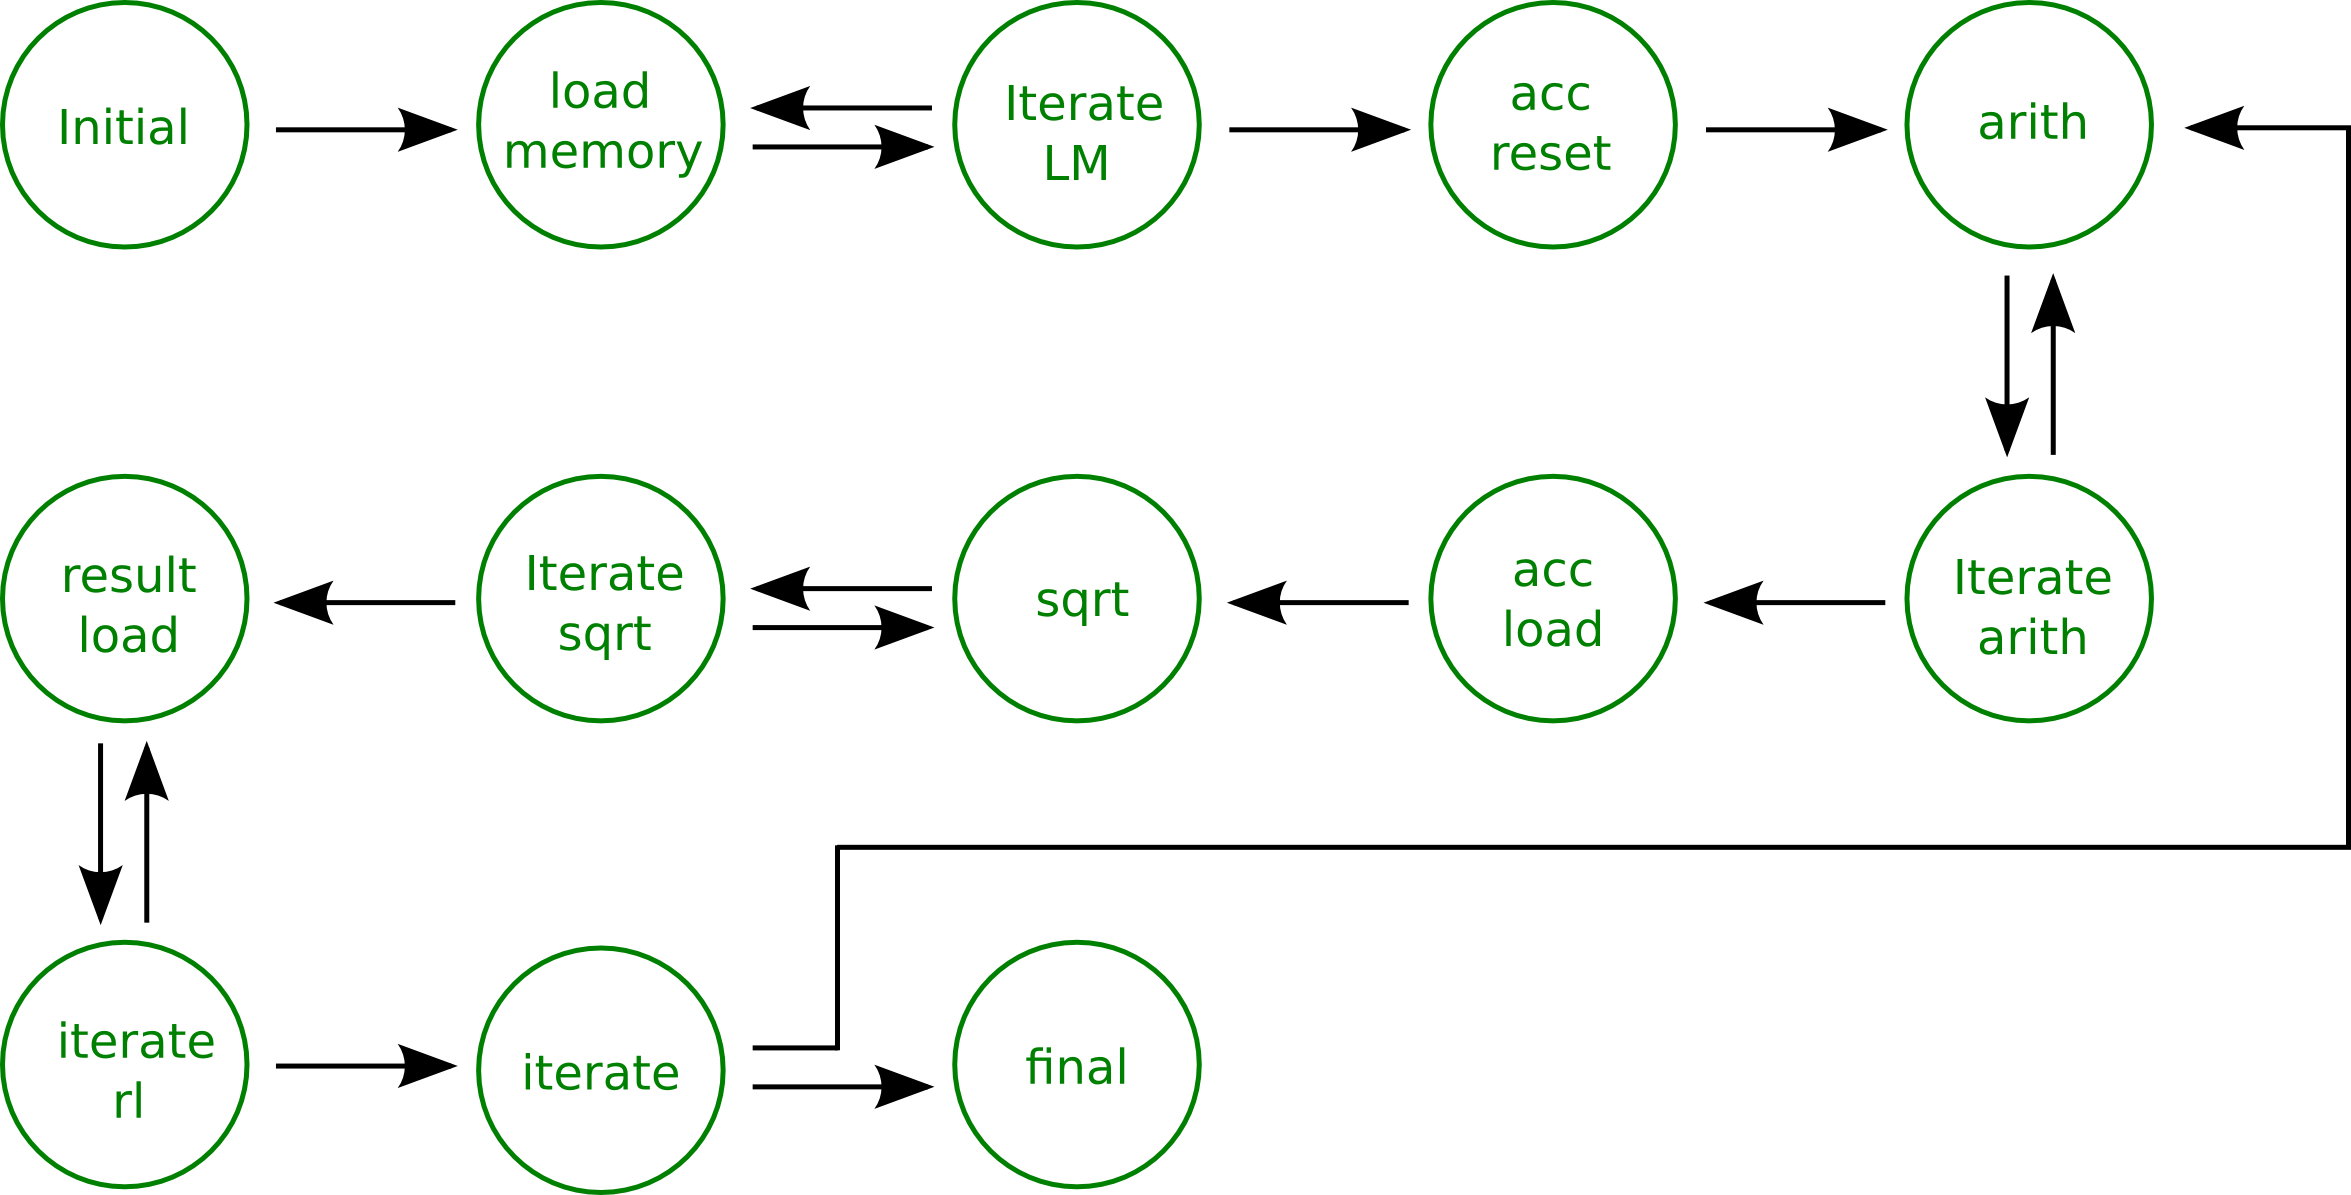
\includegraphics[scale=0.2]{img/control_unit.png}
\end{figure}
\newpage
Cada estado tem a seguinte funcionalidade:

\begin{itemize}
\item \verb|initial|: responsável por resetar as variáveis e também por esperar os dados vindos da interface com o Kinect;
\item \verb|load_memory| e \verb|iterate_lm|: Aguardam a inserção dos exemplos na memória;
\item \verb|acc_reset|: Reseta o registrador do acumulador;
\item \verb|arith| e \verb|iterate_arith|: Estado da realização das operações matemáticas das distâncias euclidianas;
\item \verb|acc_load|: Armazena a soma temporária da distância euclideana no registrador;
\item \verb|sqrt| e \verb|iterate_sqrt|: Realiza o cálculo da raiz quadrada da distância euclideana;
\item \verb|result_load| e \verb|iterate_rl|: Utiliza o componente comparador e carrega o resultado da distância euclideâna no registrador de resultado;
\item \verb|iterate|: Gerencia se o próximo estado será retornar para o ``arith'' e continuar calculando ou se já terminou os cálculos 
e deve-se ir para o estado ``final'';
\item \verb|final|: Mostra o resultado na placa e informa a interface com o KNN que a próxima entrada já pode ser enviada.
\end{itemize}


Abaixo está apresentado o bloco operativo juntamente com o bloco de controle:

\begin{figure}[!h]
\centering
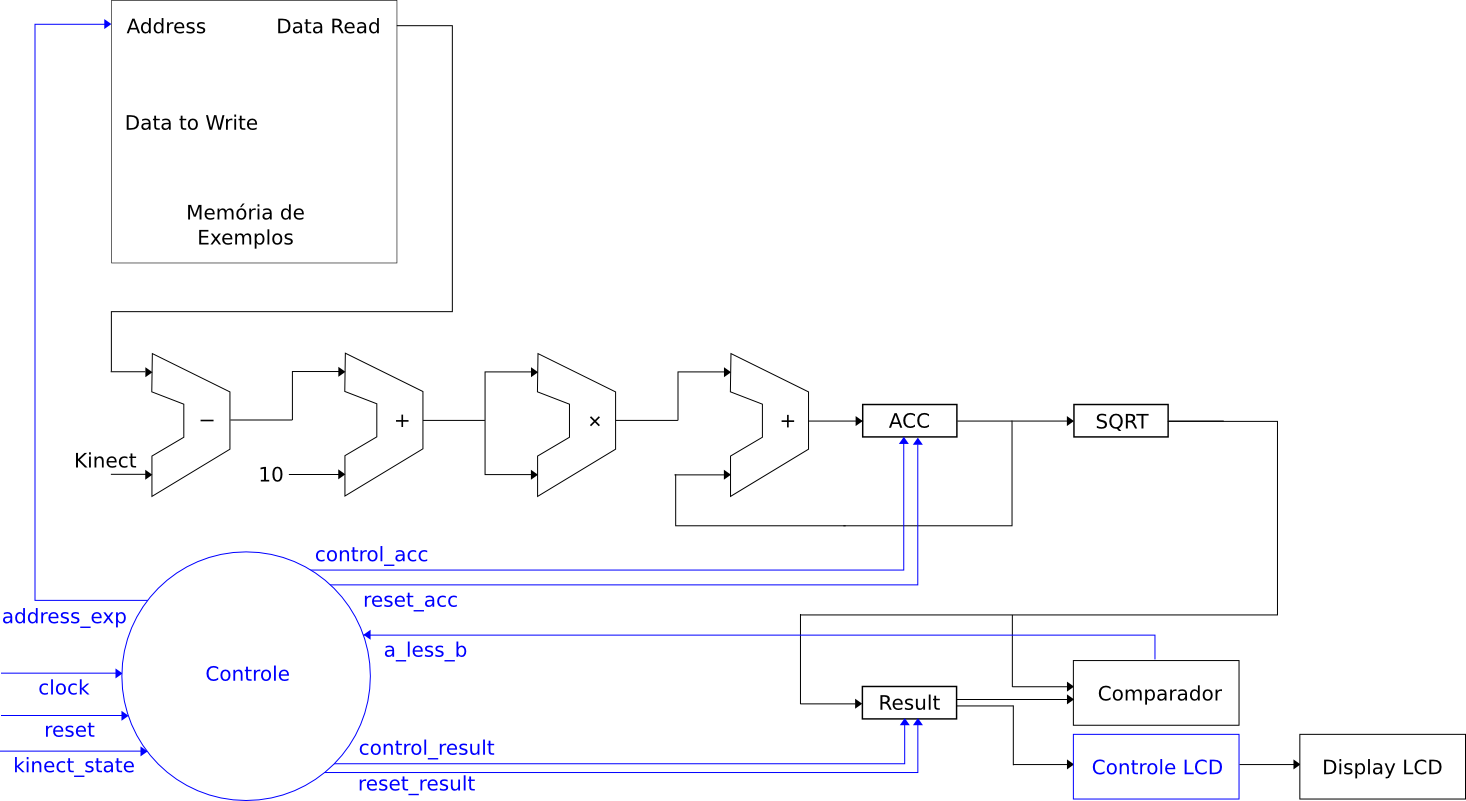
\includegraphics[scale=0.3]{img/circuito_knn.png}
\end{figure}

Descrição dos sinais do controle:

\begin{itemize}

\item \verb|adress_exp|:  Envia qual endereço da memória de exemplos deve ser acessado;
\item \verb|control_acc|: Ativa a carga no registrador acumulador no estado acc load;
\item \verb|reset_acc|: Reseta o acumulador;
\item \verb|control_result|: Ativa a carga no registrador que registra o resultado final;
\item \verb|reset_result|: Reseta o registrador;
\item \verb|kinect_state|: Sinaliza quando o exemplo vindo do kinect está pronto para ser processado;
\item \verb|a_less_b|: Resultado da comparação do valor vindo do cálculo da distância euclideana com o valor armezenado no registrador;
\end{itemize}